\documentclass[10pt]{article}
\usepackage[utf8]{inputenc}
\usepackage{pgfplots}
\pgfplotsset{compat=1.15}
\usepackage{mathrsfs}
\usetikzlibrary{arrows}
\pagestyle{empty}
\begin{document}
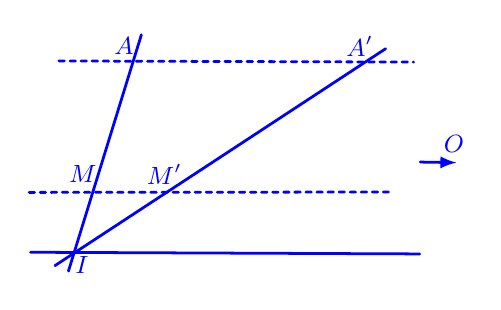
\begin{tikzpicture}[scale=1,line cap=round,line join=round,>=latex,x=1.0cm,y=1.0cm]
%\begin{axis}[x=1.0cm,y=1.0cm,axis lines=middle,ymajorgrids=true,xmajorgrids=true, xmin=0,xmax=5.5,ymin=0,ymax=3,xtick={0,1,...,5},ytick={0,1,...,3}]
%\clip(0,0) rectangle (5.5,3);
\draw [line width=1pt,color=blue] (0.017122641256603267,0.23968349948659756)-- (4.960964282672275,0.2184348964432639);
\draw [line width=1pt,color=blue] (0.5,0.)-- (1.4266133097977474,3.002001895119975);
\draw [line width=1pt,color=blue] (0.32876881922549944,0.06969467513992816)-- (4.528909354124487,2.8249302030921943);
\draw [line width=1pt,dash pattern=on 2pt off 2pt,color=blue] (0.37834889299327834,2.6691071141077476)-- (4.883052738180051,2.654941378745525);
\draw [line width=1pt,dash pattern=on 2pt off 2pt,color=blue] (0.,1.)-- (4.564323692530043,1.0046332090466097);
\draw [->,line width=1pt,color=blue] (4.9678780895883135,1.3850097751412125) -- (5.428264488860546,1.3779269074601017);
\begin{small}
\draw[color=blue] (5.395869784135131,1.611692042614109) node {$O$};
%\draw [fill=blue] (0.5732441652974685,0.23729329236321273) circle (2.0pt);
\draw[color=blue] (0.6727392429711545,0.0744575967607128) node {$I$};
%\draw [fill=blue] (0.8089185847643212,1.0008211268869986) circle (2.0pt);
\draw[color=blue] (0.6827884568885247,1.2298219137540474) node {$M$};
%\draw [fill=blue] (1.7496538092195635,1.0017760598071908) circle (2.0pt);
\draw[color=blue] (1.7178574903776516,1.2299203415887874) node {$M'$};
%\draw [fill=blue] (4.2720875381067875,2.6564585564971113) circle (2.5pt);
\draw[color=blue] (4.200013327968082,2.857794568367994) node {$A'$};
%\draw [fill=blue] (1.3232764833831212,2.6672156952540322) circle (2.5pt);
\draw[color=blue] (1.2055444362612538,2.8579914240374742) node {$A$};
\end{small}
%\end{axis}
\end{tikzpicture}
\end{document} 